\documentclass{beamer}

\usepackage{ulem}
\usepackage{amsmath}
\usepackage{mathdots}
\pagenumbering{arabic}
\usepackage{hyperref}
\usepackage{lscape}
\definecolor{slidetitlecolor}{RGB}{51,0,102}
\setbeamertemplate{footline}[frame number]%puts frame numbers in slide
\setbeamercolor{frametitle}{fg=slidetitlecolor}
\definecolor{item1color}{RGB}{51,153,255}
\setbeamercolor{itemize item}{fg=item1color}
\setbeamertemplate{itemize item}[circle]
\setbeamercolor{enumerate item}{fg=item1color}

\title{Markov Chains\vspace{-.5cm}}
\author{VK\\
Room: M1.30\\
\url{knightva@cf.ac.uk}\\
\url{www.vincent-knight.com}\\}
\date{\tiny{Last updated: \today.}}





\begin{document}

\maketitle


\frame{\frametitle{Markov Chains}\tableofcontents}
\section{Stochastic Processes and Markov Chains}
\frame{\frametitle{Stochastic Processes and Markov Chains}}
\frame{\frametitle{Stochastic Processes}
It is often possible to represent the behaviour of a system by a collection of ``states''.  An example of this could be the behaviour of the weather:\\

\begin{itemize}
\item Sunny
\item Rainy
\item Cloudy
\end{itemize}
}

\frame{\frametitle{Stochastic Processes}
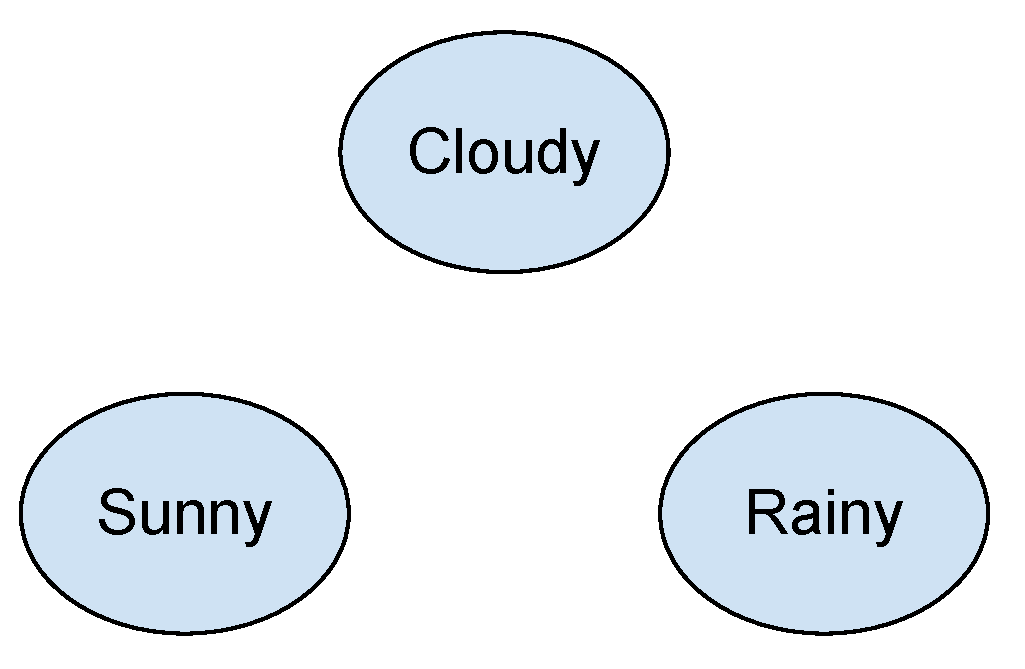
\includegraphics[width=10cm]{weather_states.pdf}
}

\section{Discrete Markov Chains}
\frame{\frametitle{Discrete Markov Chains}}

\section{Continuous Markov Chains}
\frame{\frametitle{Discrete Markov Chains}}
\end{document}
